\chapter{Transferências e sincronização dos mídias}\label{Transferências e sincronização dos mídias}\lhead{\leftmark}

\section{Transferência agendada e seletiva de arquivos}
A arquitetura do \emph{git-annex} se baseia em clones de repositórios
que sincronizam entre si os conteúdos. Pela especifica de requisitos
da RM é necessário que as operações de sincronização possam acontecer
em contextos offline. Nesses contextos os conteúdos de fato viajam
fisicamente em suportes quais laptop, HD e pendrive. O meio de
transporte dos dados é portanto baseado nas rotas físicas da
\emph{Rota dos Baobás}. As Rotas nascem de vínculos concretos
ancestrais, de afinidade, troca de produtos, encontros e vivencias,
que já existem entre as comunidades. O Baobáxia tenta aproveitar o
máximo possível as logicas e os vínculos preexistentes. 

Para entender melhor o funcionamento, detalhamos um pouco a Rota dos
Baobás a partir da Tainã, que mantém relações constantes com:
\begin{itemize}
  \item Quilombo do Cafundó (SP)
  \item Fazenda Roseira (SP)
  \item Quilombo de Brotas (SP)
  \item Mercado Sul (DF)
\end{itemize}

A Tainã e o Mercado Sul dispõem de conexão em banda larga, a Roseira
esta sem conexão internet e o Cafundó tem uma conexão por satélite.

A base da logica de triagem e circulação dos conteúdos é gerenciada
através dos ``preferred contents'' do \emph{git-annex}, que
possibilita organizar as \emph{mucuas} por grupos e definir regras de
circulação entre esses grupos, a partir de diferentes metadados (tipo
de arquivo, tag, lugar ...).

A rede do Baobáxia pode ser reconfigurada ``em andamento'', ou seja as
logicas de triagem podem mudar no tempo. Escolhemos como primeira
configuração:
\begin{table}[h]
  \centering
  \begin{tabularx}{\textwidth}{l|X| c X r X }
    \textbf{Grupo} & \textbf{Num. de copias} & \textbf{Mucuas} \\ [0.5ex]
    \hline                       
    nucleo & 1 & dandara, dpadua, exu, akoni, \ldots \\
    sync & 2 & raspberry, kalakuta-laptop, \ldots \\
    comunidade & 1 & cafundo, brotas, roseira, \ldots \\
    online & 1 & acotirene, madiba \\
    \hline  
  \end{tabularx}
\end{table}

As expressões associadas, para o \emph{nucleo}:\\
\begin{code}
(((exclude=*/archive/* and exclude=archive/*) or (not
(copies=nucleo:1 and copies=comunidade:1))) and not unused) or
roughlylackingcopies=1 or present
\end{code}

para \emph{sync}:\\
\begin{code}
(not (inallgroup=nucleo and (copies=nucleo:1 and copies=comunidade:1)) 
and ($nucleo)) or (not (inallgroup=comunidade and copies=comunidade:1)
and ($comunidade))
\end{code}

para \emph{comunidade}:\\
\begin{code}
((not (copies=comunidade:1)) and not unused) or
roughlylackingcopies=1 or present
\end{code}

para \emph{online}:\\
\begin{code}
((not (copies=online:1)) and not unused) or
roughlylackingcopies=1 or present
\end{code}



Essa configuração garante a disponibilidade dos conteúdos com 1 copia
local, 2 copias em comunidades ``próximas'', além de 2 copias em
equipamentos móveis, para circulação, e 1 copia online para acesso
através da internet.

As comunidades próximas são definidas através da configuração
dos ``remotes'' do git que no caso da Tainã são:
\begin{table}[h]
  \centering
  \begin{tabularx}{\textwidth}{ X | l  X  }
    \textbf{Mucua} & \textbf{URI} \\ [0.5ex]
    \hline
    origin & ssh://exu@acotirene.mocambos.net:/data/repositories/raiz/mocambos \\
    acotirene & ssh://exu@acotirene.mocambos.net:/data/repositories/mocambos \\
    dpadua & ssh://exu@dpadua.mocambos.net:/data/repositories/mocambos \\
    \hline  
  \end{tabularx}
\end{table}


\section{Agendamento e cron}

\section{Impulsos neurais / polinizar}
É interessante pesquisar mais as praticas de comunicação ancestrais
das comunidades, os mecanismos da natureza e aproveitar de algoritmos
de mapeamento automático de redes neurais. Imaginamos, por exemplo, um
processo exemplificado de polinização. Uma borboleta que espalha pólen
nas flores aos redores (mucuas) numa intensidade decrescente ate
acabar.

\subsection{Cibernética}
Impostamos a cibernética de polinização digital como um processo
estocástico a tempo determinado. Considerando o tamanho e os ritmos
produtivos da RM, impostamos um tempo/distancia, $t=4$. O neurônio (mucua)
$v$ ao tempo $t_{n}$ tem o impulso:

$$
x_0 = (git \ annex \ get \ \$media, ttl=4) 
$$

ao tempo $t_{1}$,

$$
x_1 = (git \ annex \ get \ \$media, ttl=3)
$$

e $t_{n+1}$,
$$
x_{n+1} = (git \ rm  \ \$thisinpulse, ttl=0)
$$

A rotina cron de sync, assumimos, conseguir uma copia do media na
mucua próxima, no tempo/distancia $t$ máxima, $ttl=4$.

\section{Gestão de conflitos entre versões}

O impulso pode ser codificado como arquivo json com nome aleatório
($date\_UUID[:5]$) que cada mucua mantém numa pasta de solicitações
(ex. $mocambos/dpadua/semeando/$):

\begin{code}
  {"mediafile" : "$path", "ttl" : "4" }
\end{code}

Isso garante a falta de conflitos entre arquivos porque cada mucua
altera seus impulsos. A cada ciclo de cron, e sob determinadas
condições, a mucua consulta os impulsos das outras próximas (ver
rotas/remotes) e copia os impulsos reduzindo o peso, de fato
propagando o impulso.

Os impulsos decaem e os arquivos são removidos quando as mucuas
conseguem uma copia do media.  

\section{Sincronização do git}
além de git annex sync , git pull \& push

\section{Teoria estocástica}

$P(X(n))$, \ Probabilidade de encontrar o media ao tempo/passo n.

$$
P(x_n<=x_{n+1} | P(x_n)=x_n)
$$

Com, $P(x_0)=0$, $P(x_{n+1})=1$ e:

$$
P(X_{n+1}) = P(X_n)+P(x_{n-1})
$$







%% \subsection{Git}\label{sec:GIT}

%% \item suporta o \emph{branching} (ramificação), e o \emph{merging}
%%   (fusão), de maneira rápida e conveniente, incluindo uma serie de
%%   ferramentas para visualizar e navegar o histórico não linear das
%%   versões.


%% \begin{figure}[htbp]
%%   \centering
%%   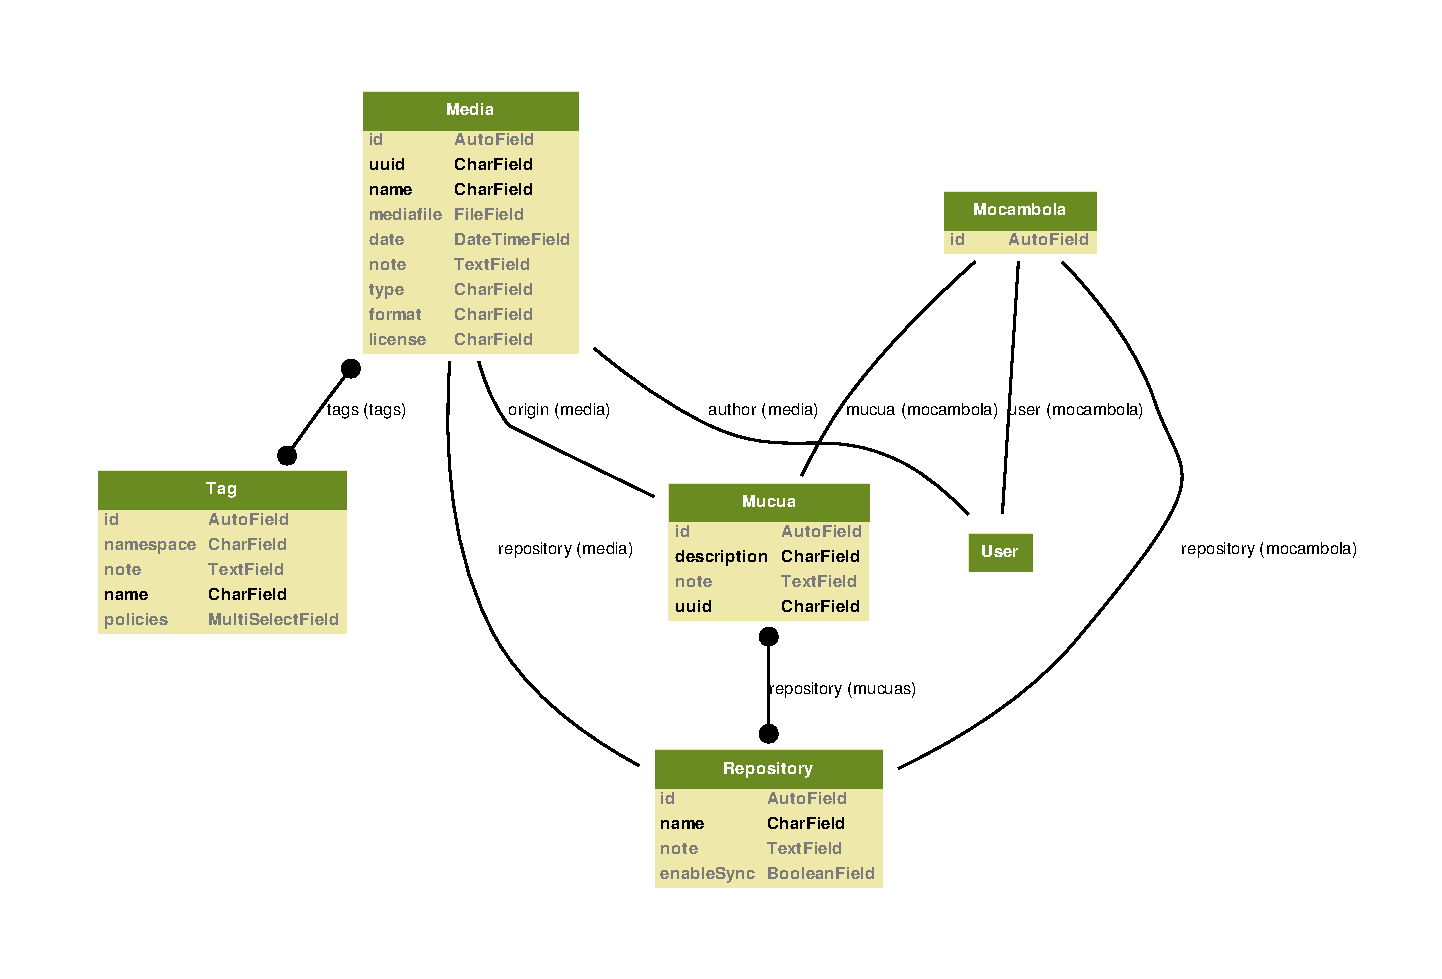
\includegraphics[width=\textwidth]{./Fig/Auto_UML_Diagram.pdf}
%%   \rule{35em}{0.5pt}
%%   \caption[Diagrama UML do BBX]{Diagrama UML do BBX}
%%   \label{fig:SchemaServer_ReteMocambos}
%% \end{figure}

